\documentclass{beamer}
\usepackage{graphicx}
\usepackage[spanish]{babel}
\usepackage{amsmath}

\title{Determinación Teórica del Salario Mínimo en Perú}
\author{}
\institute{}
\date{\today}

\begin{document}

% Diapositiva 1: Título
\begin{frame}
    \titlepage
\end{frame}

% Diapositiva 4: Aplicación al Caso de Perú
\begin{frame}{Recientemente se propuso que el salario mínimo sea 726 soles...}
    \begin{center}
        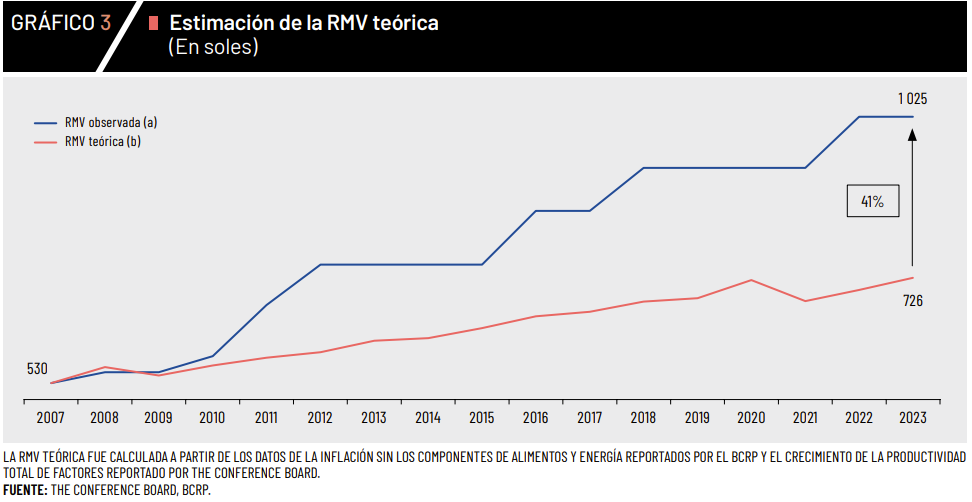
\includegraphics[width=\linewidth]{bcrp_salmin.PNG}
    \end{center}
\end{frame}


% Diapositiva 2: Explicación del Enfoque
\begin{frame}{¿Qué supuestos tiene esta estimación?}
    \begin{itemize}
        \item \textbf{Supuestos:} Los cambios en el salario mínimo se consideran iguales a las variaciones en la inflación y la productividad bajo una teoría simplificada.
        \item \textbf{Inflación:} Se usa la inflación subyacente de Lima Metropolitana. No obstante, es mejor usar la inflación nacional porque incluye todos los bienes y servicios consumidos por los trabajadores a nivel nacional, reflejando más fielmente el costo de vida real.
        \item \textbf{Productividad:} Se utiliza la productividad total de los factores (PTF). Es mejor usar la productividad laboral (PL) porque refleja directamente el valor económico generado por cada trabajador.
        \item \textbf{Teoría simplificada:} Este enfoque ignora el poder monopsonístico en el mercado laboral.
    \end{itemize}
\end{frame}

% Diapositiva 3: Derivación del Salario en Mercados Laborales Imperfectos
\begin{frame}{¿Cuál debería ser la forma de estimar el cambio en el salario mínimo?}
    \textbf{En mercados laborales con poder monopsónico (Borjas, 2013), la teoría económica postula que:}
    \begin{align*}
        \text{Maximización del beneficio:} \quad & \pi = P \cdot f(L) - w \cdot L \\
        \text{Condición de primer orden:} \quad & P \cdot f'(L) = w + \frac{\partial w}{\partial L} L \\
        \text{Salario óptimo:} \quad & w = P \cdot \text{MPL} \cdot \left( 1 + \frac{1}{e_s} \right) \\
        \text{Logs y diferenciando:} \quad & \Delta w = \Delta P + \Delta \text{MPL} + \frac{\Delta {e_s}}{1+e_s}
    \end{align*}
    Donde:
    \begin{itemize}
        \item $P$: precio del producto
        \item $\text{MPL}$: productividad marginal del trabajo.
        \item $e_s$: elasticidad de la oferta laboral.
    \end{itemize}
\end{frame}

% Diapositiva 4: Aplicación al Caso de Perú
\begin{frame}{Replicando el análisis sin considerar que el mercado laboral es concentrado:}
    \begin{center}
        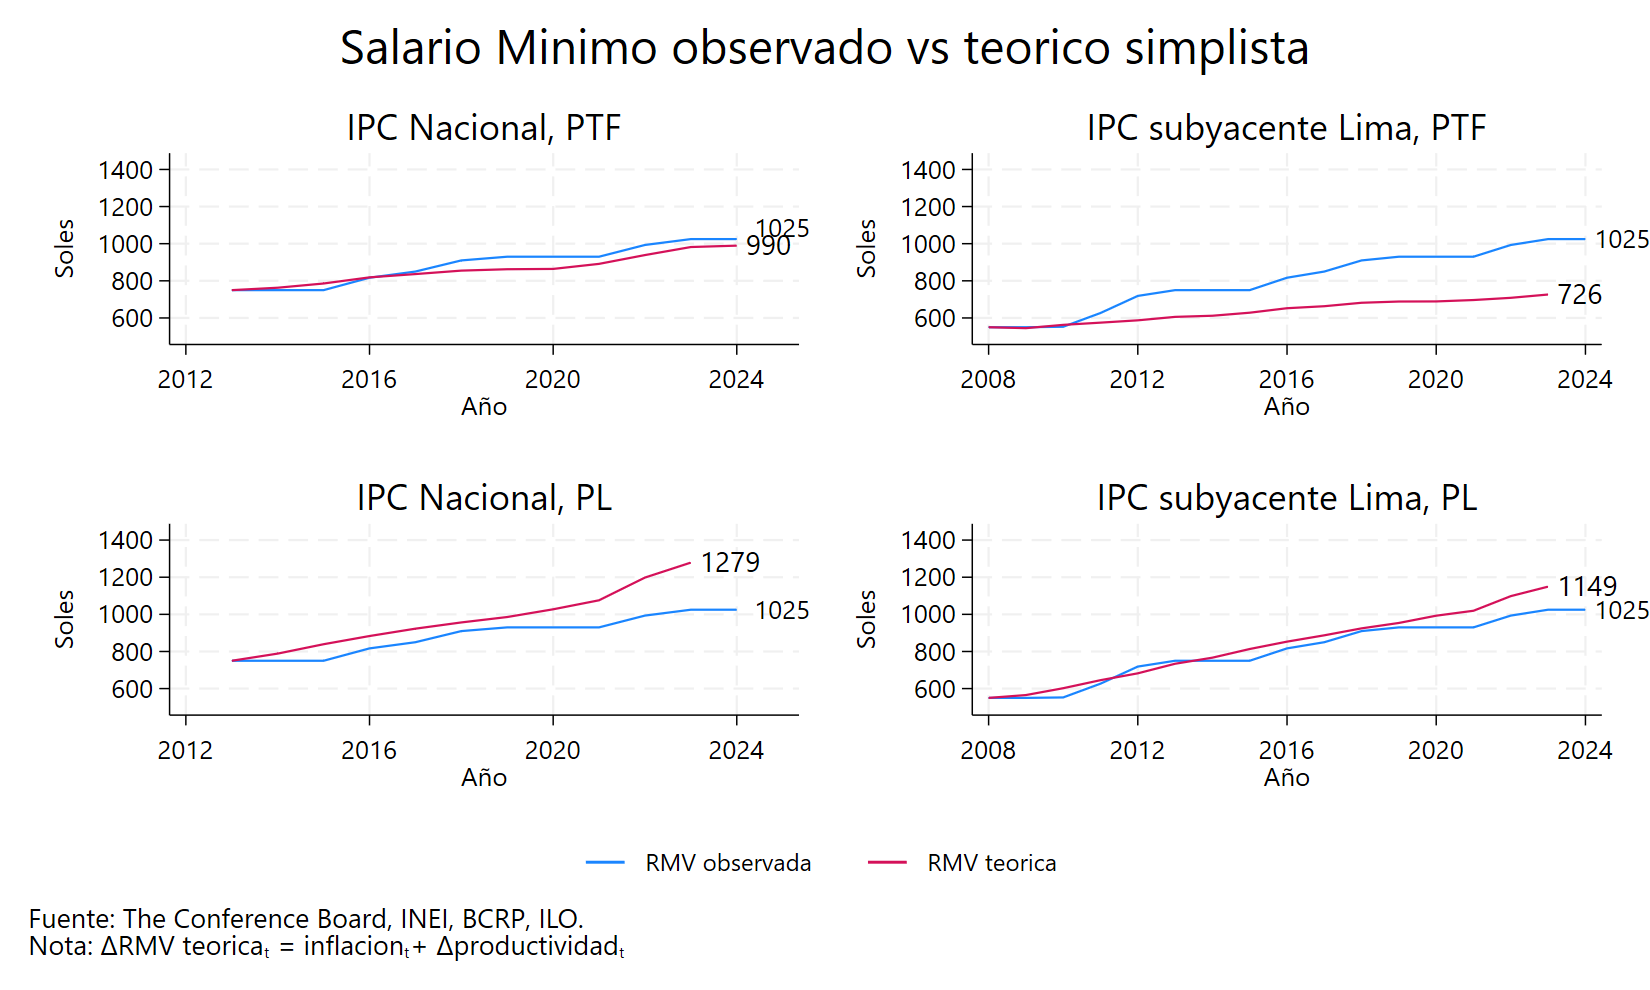
\includegraphics[width=\linewidth]{rmv_determination_sine.png}
    \end{center}
\end{frame}

% Diapositiva 4: Aplicación al Caso de Perú
\begin{frame}{Sin embargo, al usar la teoría que considera mercados laborales concentrados, se observa que el salario mínimo esta por debajo del nivel que debería estar:}
    \begin{center}
        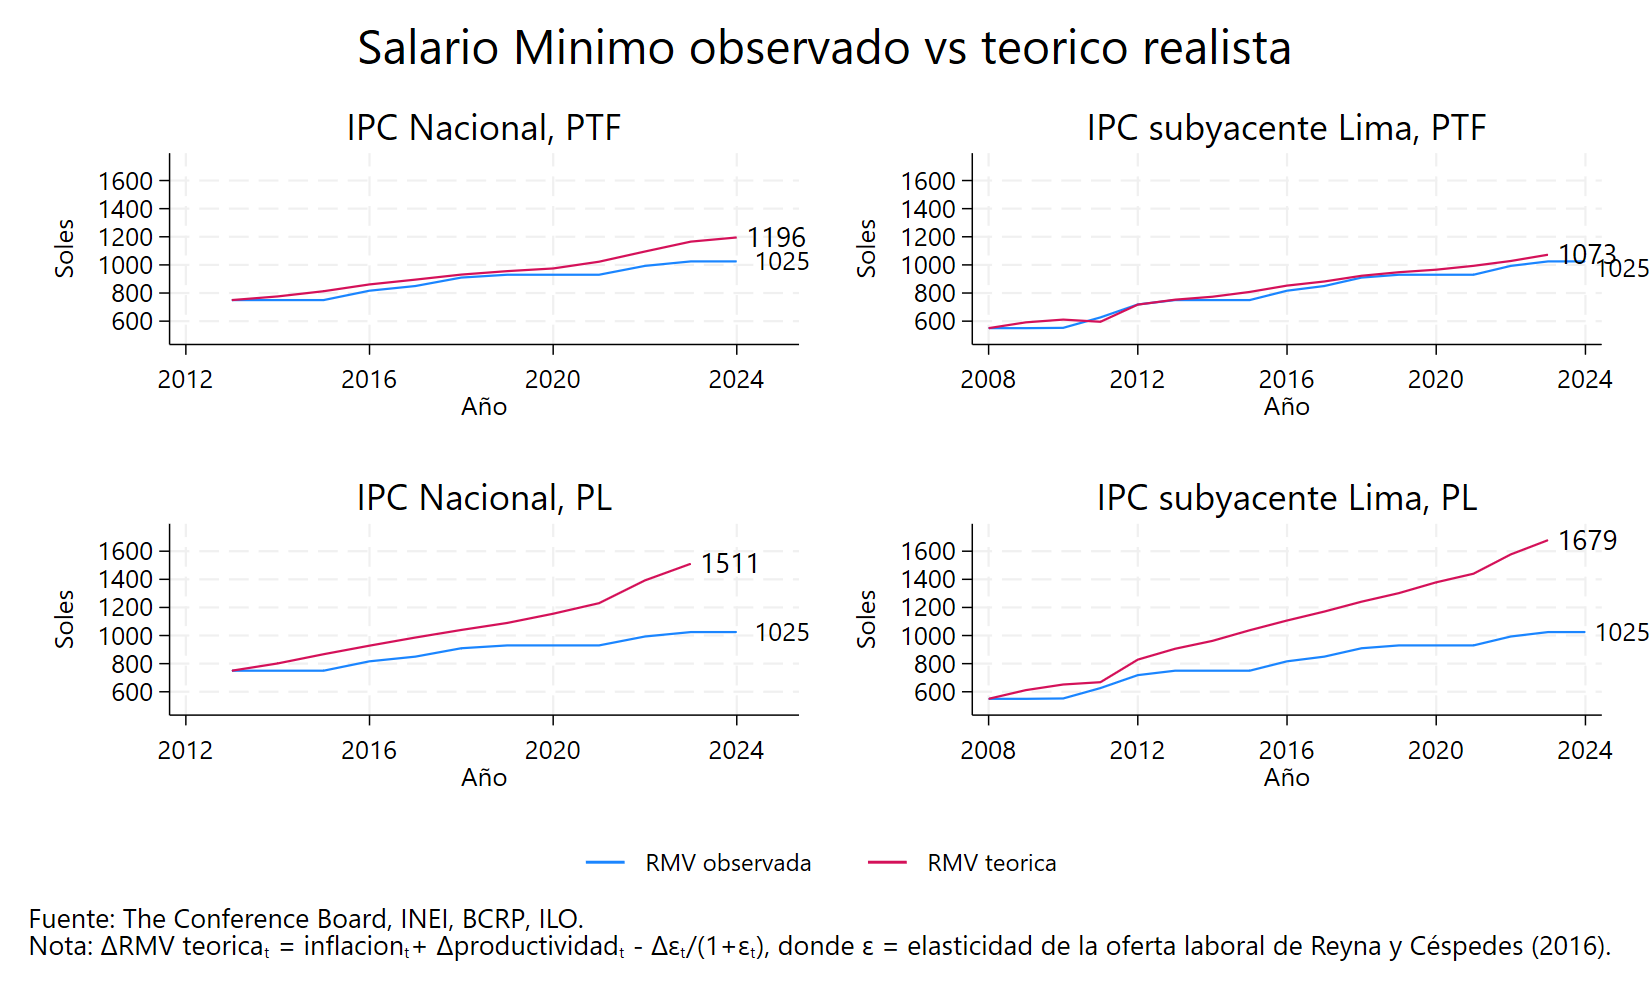
\includegraphics[width=\linewidth]{rmv_determination_cone.png}
    \end{center}
\end{frame}

\end{document}
